% Options for packages loaded elsewhere
\PassOptionsToPackage{unicode}{hyperref}
\PassOptionsToPackage{hyphens}{url}
%
\documentclass[
  ignorenonframetext,
]{beamer}
\usepackage{pgfpages}
\setbeamertemplate{caption}[numbered]
\setbeamertemplate{caption label separator}{: }
\setbeamercolor{caption name}{fg=normal text.fg}
\beamertemplatenavigationsymbolsempty
% Prevent slide breaks in the middle of a paragraph
\widowpenalties 1 10000
\raggedbottom
\setbeamertemplate{part page}{
  \centering
  \begin{beamercolorbox}[sep=16pt,center]{part title}
    \usebeamerfont{part title}\insertpart\par
  \end{beamercolorbox}
}
\setbeamertemplate{section page}{
  \centering
  \begin{beamercolorbox}[sep=12pt,center]{part title}
    \usebeamerfont{section title}\insertsection\par
  \end{beamercolorbox}
}
\setbeamertemplate{subsection page}{
  \centering
  \begin{beamercolorbox}[sep=8pt,center]{part title}
    \usebeamerfont{subsection title}\insertsubsection\par
  \end{beamercolorbox}
}
\AtBeginPart{
  \frame{\partpage}
}
\AtBeginSection{
  \ifbibliography
  \else
    \frame{\sectionpage}
  \fi
}
\AtBeginSubsection{
  \frame{\subsectionpage}
}

\usepackage{amsmath,amssymb}
\usepackage{lmodern}
\usepackage{iftex}
\ifPDFTeX
  \usepackage[T1]{fontenc}
  \usepackage[utf8]{inputenc}
  \usepackage{textcomp} % provide euro and other symbols
\else % if luatex or xetex
  \usepackage{unicode-math}
  \defaultfontfeatures{Scale=MatchLowercase}
  \defaultfontfeatures[\rmfamily]{Ligatures=TeX,Scale=1}
\fi
% Use upquote if available, for straight quotes in verbatim environments
\IfFileExists{upquote.sty}{\usepackage{upquote}}{}
\IfFileExists{microtype.sty}{% use microtype if available
  \usepackage[]{microtype}
  \UseMicrotypeSet[protrusion]{basicmath} % disable protrusion for tt fonts
}{}
\makeatletter
\@ifundefined{KOMAClassName}{% if non-KOMA class
  \IfFileExists{parskip.sty}{%
    \usepackage{parskip}
  }{% else
    \setlength{\parindent}{0pt}
    \setlength{\parskip}{6pt plus 2pt minus 1pt}}
}{% if KOMA class
  \KOMAoptions{parskip=half}}
\makeatother
\usepackage{xcolor}
\newif\ifbibliography
\setlength{\emergencystretch}{3em} % prevent overfull lines
\setcounter{secnumdepth}{-\maxdimen} % remove section numbering


\providecommand{\tightlist}{%
  \setlength{\itemsep}{0pt}\setlength{\parskip}{0pt}}\usepackage{longtable,booktabs,array}
\usepackage{calc} % for calculating minipage widths
\usepackage{caption}
% Make caption package work with longtable
\makeatletter
\def\fnum@table{\tablename~\thetable}
\makeatother
\usepackage{graphicx}
\makeatletter
\def\maxwidth{\ifdim\Gin@nat@width>\linewidth\linewidth\else\Gin@nat@width\fi}
\def\maxheight{\ifdim\Gin@nat@height>\textheight\textheight\else\Gin@nat@height\fi}
\makeatother
% Scale images if necessary, so that they will not overflow the page
% margins by default, and it is still possible to overwrite the defaults
% using explicit options in \includegraphics[width, height, ...]{}
\setkeys{Gin}{width=\maxwidth,height=\maxheight,keepaspectratio}
% Set default figure placement to htbp
\makeatletter
\def\fps@figure{htbp}
\makeatother

\makeatletter
\makeatother
\makeatletter
\makeatother
\makeatletter
\@ifpackageloaded{caption}{}{\usepackage{caption}}
\AtBeginDocument{%
\ifdefined\contentsname
  \renewcommand*\contentsname{Table of contents}
\else
  \newcommand\contentsname{Table of contents}
\fi
\ifdefined\listfigurename
  \renewcommand*\listfigurename{List of Figures}
\else
  \newcommand\listfigurename{List of Figures}
\fi
\ifdefined\listtablename
  \renewcommand*\listtablename{List of Tables}
\else
  \newcommand\listtablename{List of Tables}
\fi
\ifdefined\figurename
  \renewcommand*\figurename{Figure}
\else
  \newcommand\figurename{Figure}
\fi
\ifdefined\tablename
  \renewcommand*\tablename{Table}
\else
  \newcommand\tablename{Table}
\fi
}
\@ifpackageloaded{float}{}{\usepackage{float}}
\floatstyle{ruled}
\@ifundefined{c@chapter}{\newfloat{codelisting}{h}{lop}}{\newfloat{codelisting}{h}{lop}[chapter]}
\floatname{codelisting}{Listing}
\newcommand*\listoflistings{\listof{codelisting}{List of Listings}}
\makeatother
\makeatletter
\@ifpackageloaded{caption}{}{\usepackage{caption}}
\@ifpackageloaded{subcaption}{}{\usepackage{subcaption}}
\makeatother
\makeatletter
\@ifpackageloaded{tcolorbox}{}{\usepackage[many]{tcolorbox}}
\makeatother
\makeatletter
\@ifundefined{shadecolor}{\definecolor{shadecolor}{rgb}{.97, .97, .97}}
\makeatother
\makeatletter
\makeatother
\ifLuaTeX
  \usepackage{selnolig}  % disable illegal ligatures
\fi
\IfFileExists{bookmark.sty}{\usepackage{bookmark}}{\usepackage{hyperref}}
\IfFileExists{xurl.sty}{\usepackage{xurl}}{} % add URL line breaks if available
\urlstyle{same} % disable monospaced font for URLs
\hypersetup{
  pdftitle={Support Vector Machines},
  pdfauthor={Robert Belina},
  hidelinks,
  pdfcreator={LaTeX via pandoc}}

\title{Support Vector Machines}
\author{Robert Belina}
\date{}

\begin{document}
\frame{\titlepage}
\ifdefined\Shaded\renewenvironment{Shaded}{\begin{tcolorbox}[breakable, borderline west={3pt}{0pt}{shadecolor}, enhanced, boxrule=0pt, interior hidden, frame hidden, sharp corners]}{\end{tcolorbox}}\fi

\begin{frame}{Introduction}
\protect\hypertarget{introduction}{}
Support Vector Machines (SVMs) have emerged as a powerful and versatile
machine learning algorithm with applications spanning various domains.
Developed by Vapnik and colleagues in the 1990s, SVMs have gained
significant popularity due to their ability to handle both
classification and regression tasks effectively. The fundamental concept
behind SVMs is to find an optimal hyperplane that maximally separates
different classes or fits the data points for regression, while
simultaneously maintaining a clear margin between them
{[}@kecman\_2005\_support{]}.

\begin{block}{Brief Introduction to Machine Learning}
\protect\hypertarget{brief-introduction-to-machine-learning}{}
Machine learning is the process of enabling computers to take actions by
providing them with data and allowing them to discover patterns and
insights autonomously, without explicit programming.

At the core of machine learning lies the importance of data. Just as
humans learn through information and data gathering, machines also
require data to learn and make informed decisions.

\begin{figure}

{\centering 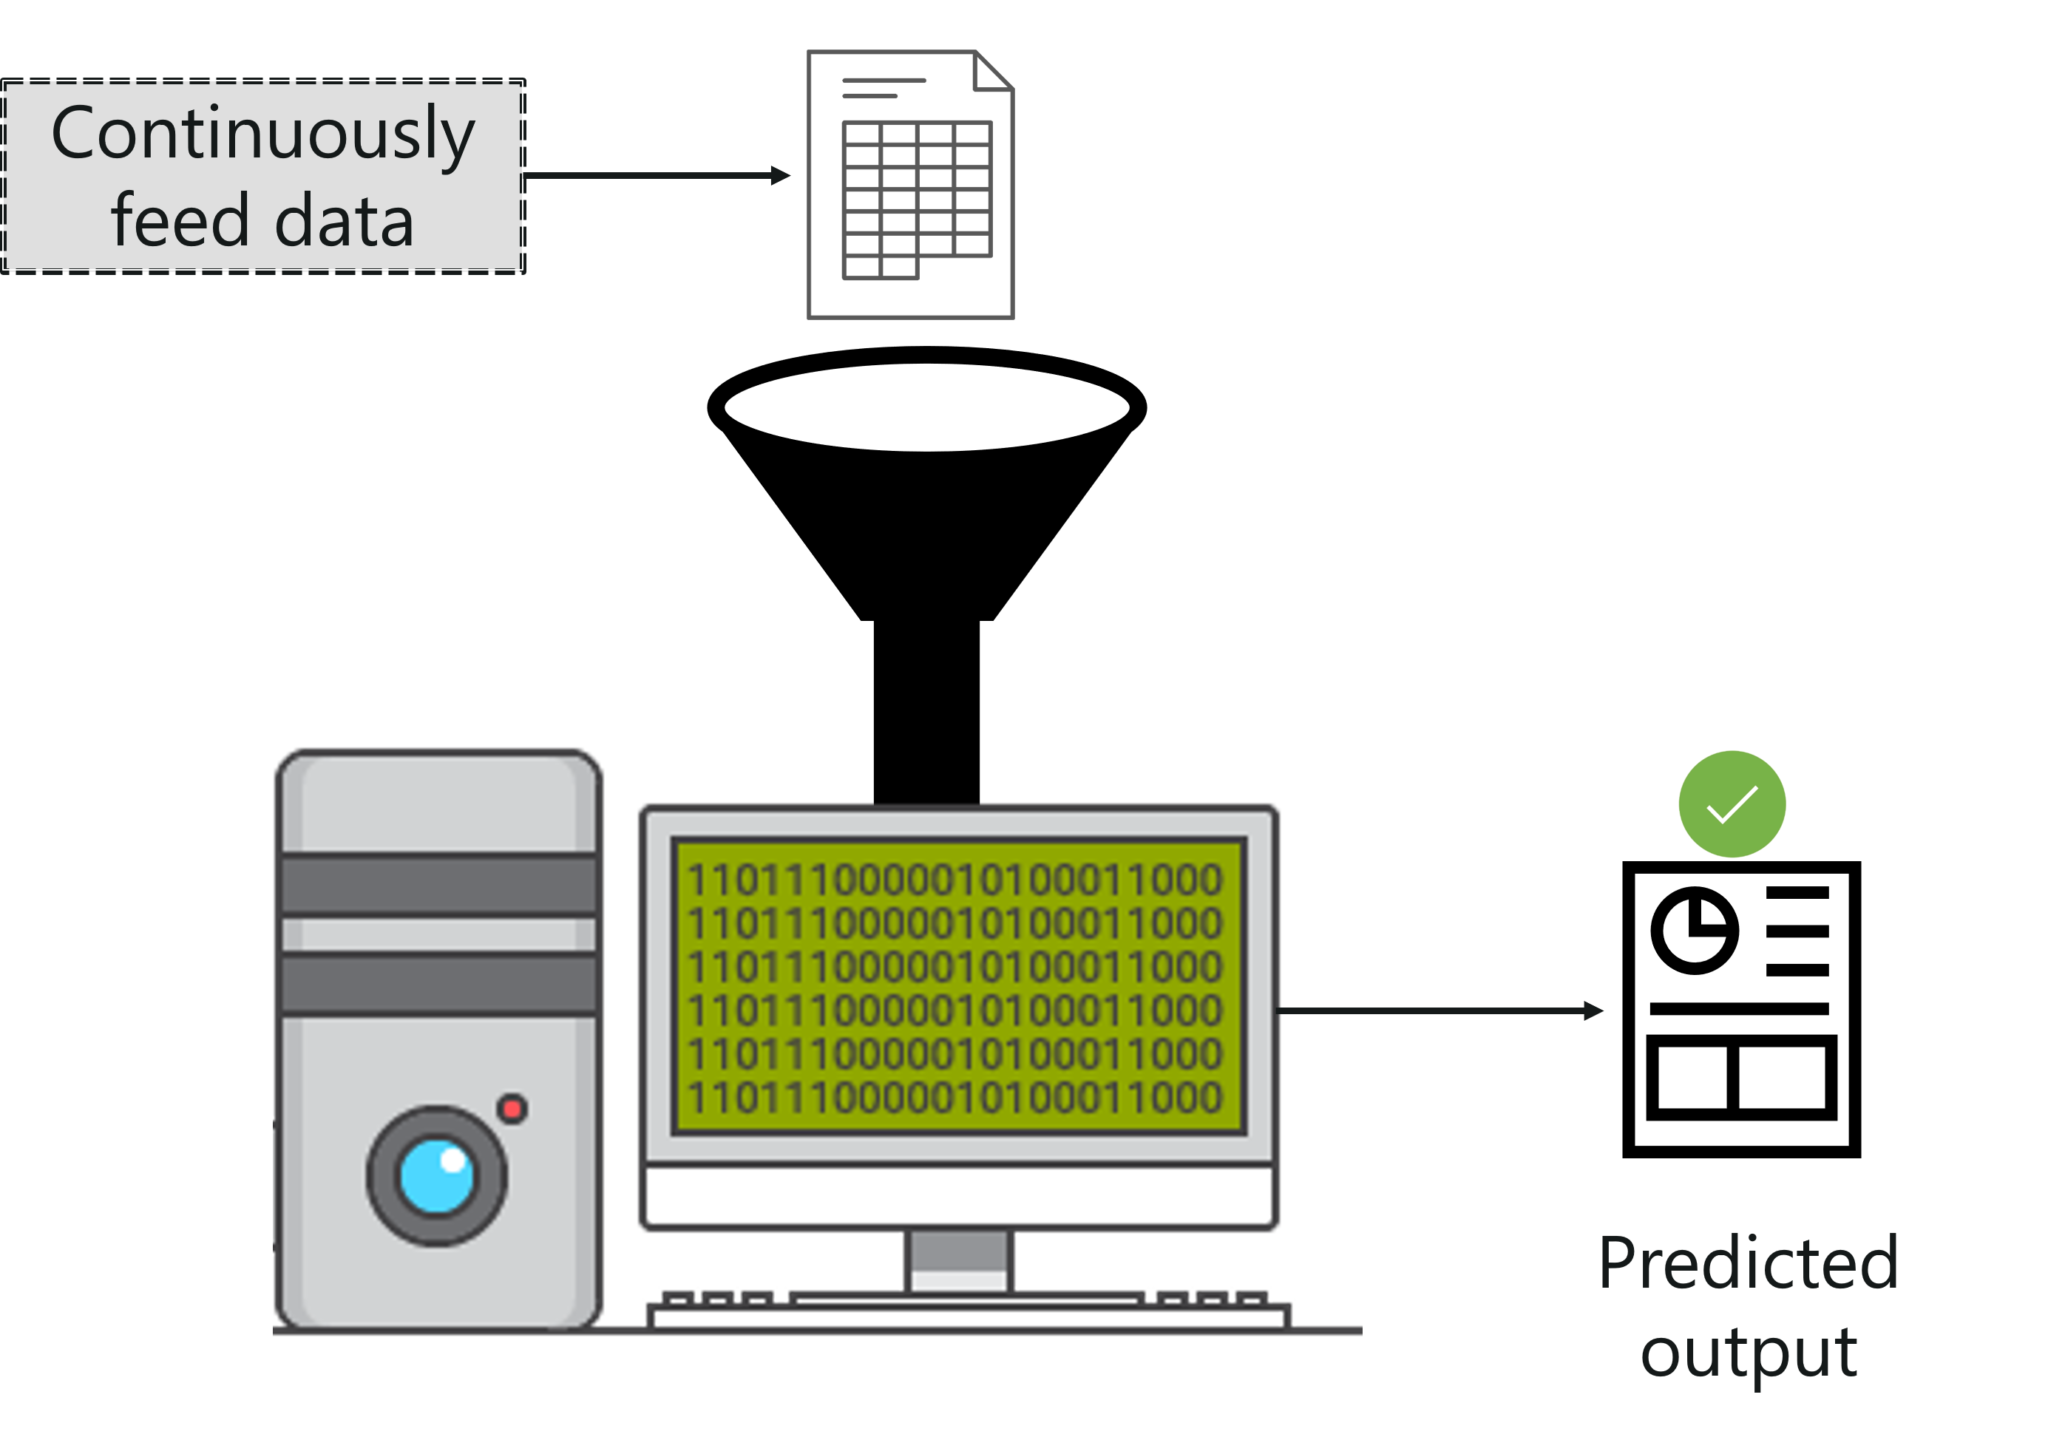
\includegraphics{ml1.png}

}

\caption{citation}

\end{figure}

SVMs offer several advantages over traditional classification
algorithms. Unlike methods that solely focus on minimizing training
errors, SVMs are designed to maximize the margin between classes. This
margin not only aids in achieving robust and accurate predictions on
unseen data but also enhances the generalization ability of the model.
By emphasizing the importance of the margin, SVMs can effectively handle
datasets with high dimensionality, noise, and outliers, resulting in
superior performance in complex scenarios {[}@tian\_2012\_recent{]}.

The distinguishing feature of SVMs lies in their ability to transform
the original input space into a higher-dimensional feature space through
the use of kernel functions. This enables SVMs to handle nonlinear
relationships between variables without explicitly mapping them into the
higher-dimensional space. By leveraging the kernel trick, SVMs
efficiently capture complex decision boundaries, offering flexibility
and adaptability to various data distributions. Furthermore, SVMs
provide a principled approach to handle both binary and multiclass
classification problems. Through techniques such as one-vs-one and
one-vs-all, SVMs can extend their capabilities to accommodate multiple
classes, ensuring accurate predictions across diverse scenarios
{[}@evgenybyvatov\_2003\_support{]}

The versatility of SVMs extends beyond classification tasks, as they
have also been successfully applied to regression, anomaly detection,
and outlier detection problems. By employing support vector regression
(SVR), SVMs can capture nonlinear relationships in continuous variables,
making them well-suited for prediction tasks involving numerical outputs
{[}@brereton\_2010\_support{]}.

In this review, we aim to provide an in-depth exploration of Support
Vector Machines, covering their fundamental concepts, mathematical
foundations, training algorithms, and diverse applications across
various fields. By understanding the underlying principles and
techniques of SVMs, researchers and practitioners can effectively
leverage thi\$\$s powerful tool to tackle complex classification and
regression problems, ultimately leading to enhanced predictive accuracy
and insightful data analysis {[}@yang\_2004\_biological{]}.
\end{block}
\end{frame}

\begin{frame}{Methods}
\protect\hypertarget{methods}{}
To begin understanding the usecases of SVMs we will first look at the
underlying math behind SVMs: linear algebra and a touch of optimization
theory.

\begin{block}{Definintions}
\protect\hypertarget{definintions}{}
\emph{Length of a Vector}

The norm of a vector x, denoted as \textbar\textbar x\textbar\textbar,
represents its length. The Euclidean norm formula used to compute the
norm of a vector x = (x1, x2, \ldots, xn) is as follows:

\[
||x||= √x21+x22+...+x2n
\]

\emph{Vector Directions}

The direction of a vector x = (x1, x2) is denoted by w and is defined as
follows:

\(w = (x1/||x||,x2/||x||)\)

Looking at the above, we can view the direction of the vector \emph{w}
as:

\begin{figure}

{\centering 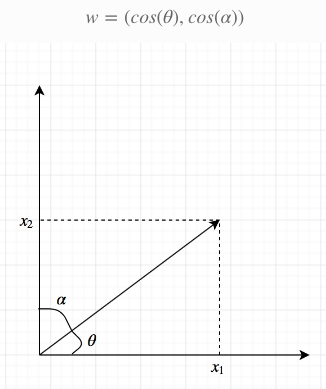
\includegraphics{ml2.png}

}

\caption{citation}

\end{figure}

Support Vector Machines (SVMs) are a robust machine learning algorithm
used for classification and regression tasks. In this section, we
describe the key steps involved in implementing SVMs, including data
preprocessing, model training, and model evaluation.

Data Preprocessing:

Data Cleaning: Remove any irrelevant or redundant features, handle
missing values, and address outliers if necessary. Feature Scaling:
Normalize the feature values to ensure that they have similar scales.
Common scaling techniques include standardization (mean centering and
scaling to unit variance) or normalization to a specific range. Feature
Selection: Select relevant features that contribute most to the
prediction task, reducing dimensionality and improving model
performance. Data Split: Divide the dataset into training and testing
subsets. The training set is used to train the SVM model, while the
testing set is used for evaluating its performance. Model Training:

Kernel Selection: Determine the appropriate kernel function based on the
nature of the data and the problem at hand. Common kernel functions
include linear, polynomial, Gaussian radial basis function (RBF), and
sigmoid. Hyperparameter Tuning: Optimize the hyperparameters of the SVM
model, such as the regularization parameter C and kernel-specific
parameters like the degree of polynomial or the width of the RBF kernel.
This can be done using techniques like grid search or cross-validation.
Model Fitting: Train the SVM model using the training dataset and the
chosen hyperparameters. The goal is to find the optimal hyperplane or
decision boundary that maximizes the margin between classes (in the case
of classification) or minimizes the error (in the case of regression).
Model Evaluation:

Classification Metrics: Evaluate the performance of the SVM model for
classification tasks using metrics such as accuracy, precision, recall,
F1-score, and area under the receiver operating characteristic curve
(AUC-ROC). Regression Metrics: Assess the performance of the SVM model
for regression tasks using metrics such as mean squared error (MSE),
root mean squared error (RMSE), mean absolute error (MAE), and
R-squared. Cross-Validation: Perform k-fold cross-validation to estimate
the model's generalization performance. This involves dividing the
training dataset into k subsets, training the model on k-1 subsets, and
evaluating its performance on the remaining subset. Repeat this process
k times, rotating the evaluation subset each time. Model Selection:
Compare the performance of different SVM models with varying
hyperparameters or kernel functions to select the optimal model with the
best performance on the testing dataset. Model Deployment:

Once the SVM model has been trained and evaluated, it can be deployed to
make predictions on new, unseen data. Preprocess the new data using the
same steps as the training data (e.g., feature scaling), and apply the
trained SVM model to classify or regress the new instances.
\end{block}
\end{frame}

\begin{frame}[fragile]{Analysis and Results}
\protect\hypertarget{analysis-and-results}{}
\begin{block}{Linear Support Vector Machine Classifier}
\protect\hypertarget{linear-support-vector-machine-classifier}{}
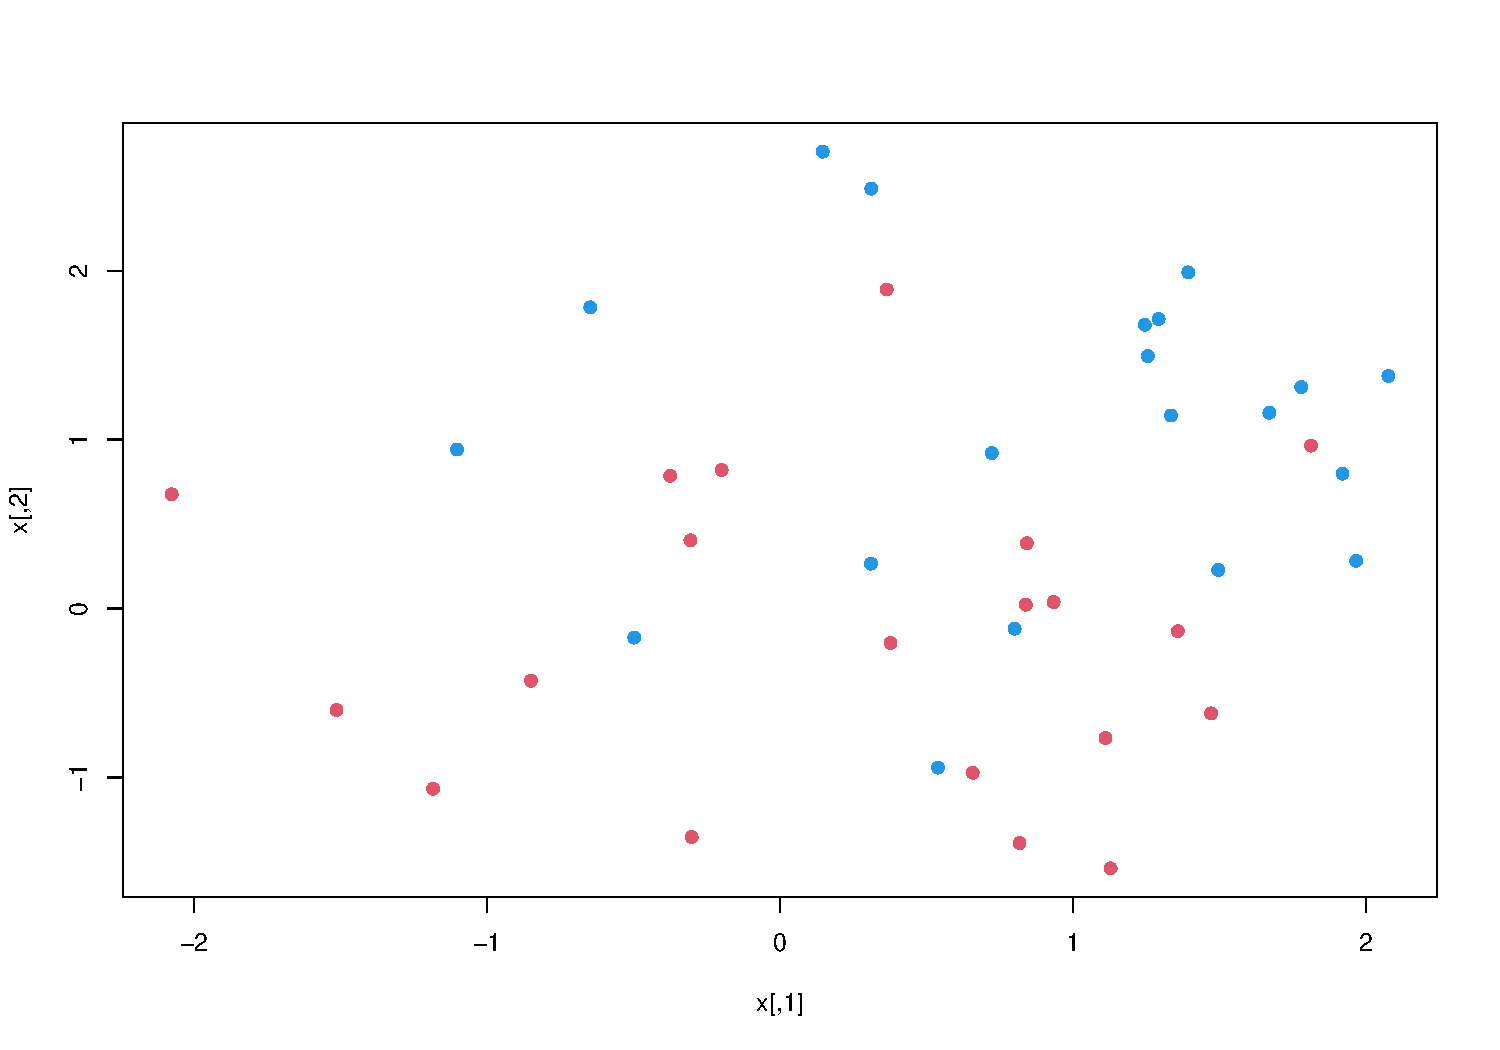
\includegraphics{slides_files/figure-beamer/unnamed-chunk-1-1.pdf}

\begin{verbatim}

Call:
svm(formula = y ~ ., data = dat, kernel = "linear", cost = 10, scale = FALSE)


Parameters:
   SVM-Type:  C-classification 
 SVM-Kernel:  linear 
       cost:  10 

Number of Support Vectors:  23
\end{verbatim}

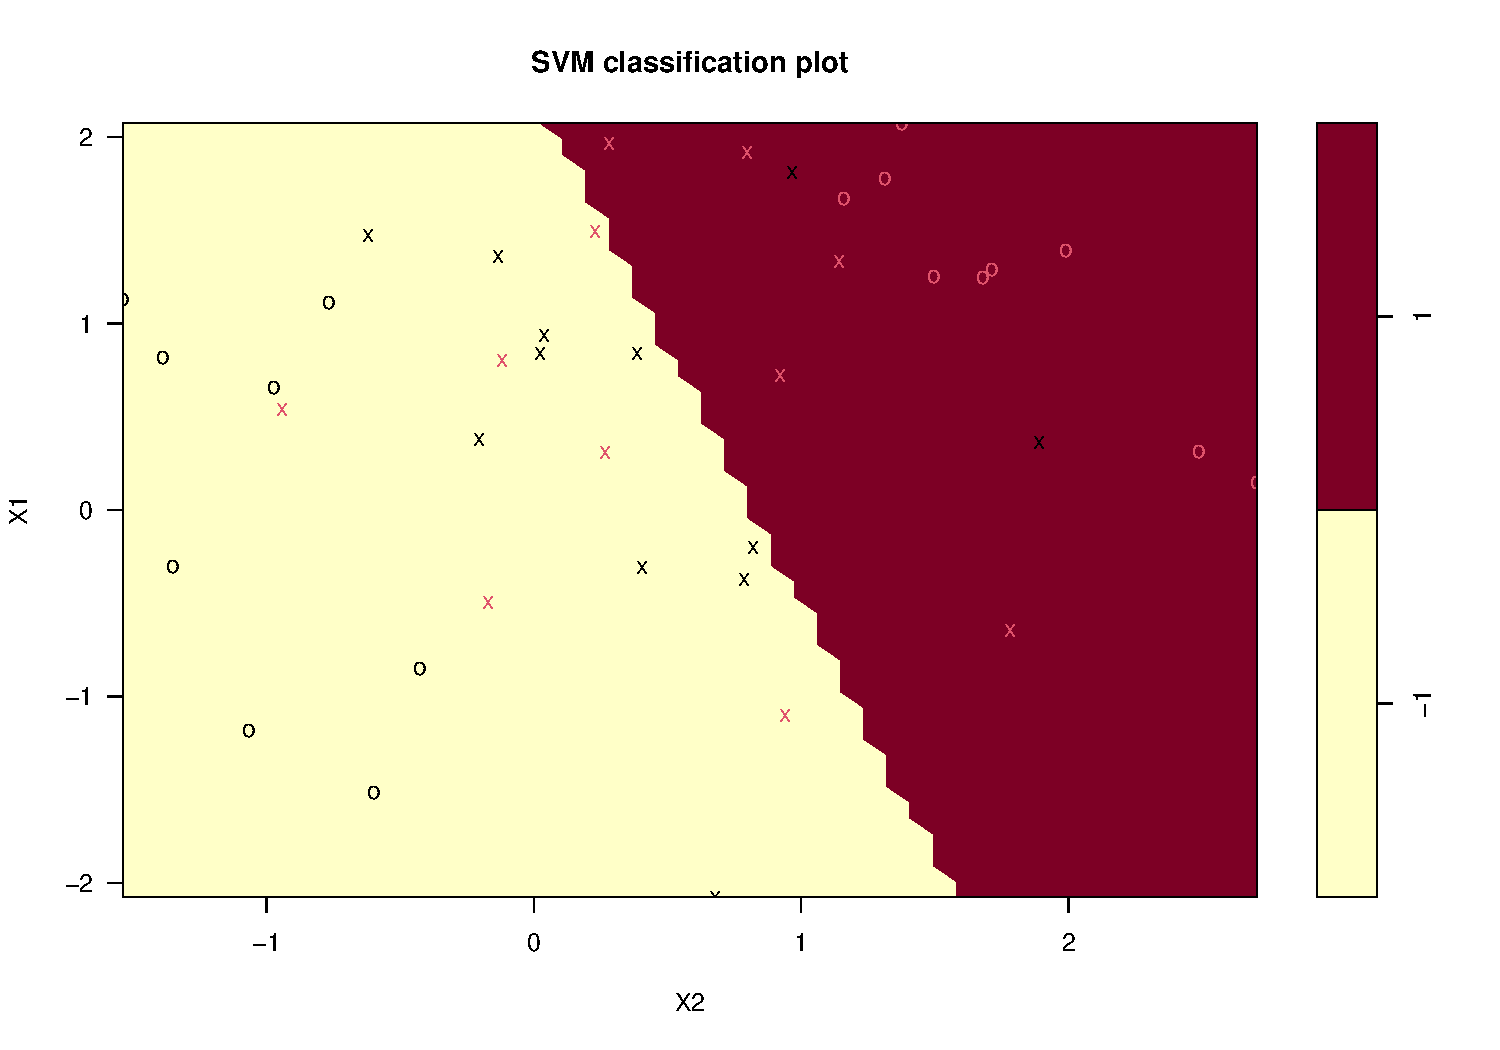
\includegraphics{slides_files/figure-beamer/unnamed-chunk-1-2.pdf}

\begin{verbatim}
          X1        X2
1  -2.075718 -1.536734
2  -2.035796 -1.536734
3  -1.995873 -1.536734
4  -1.955950 -1.536734
5  -1.916028 -1.536734
6  -1.876105 -1.536734
7  -1.836183 -1.536734
8  -1.796260 -1.536734
9  -1.756337 -1.536734
10 -1.716415 -1.536734
\end{verbatim}

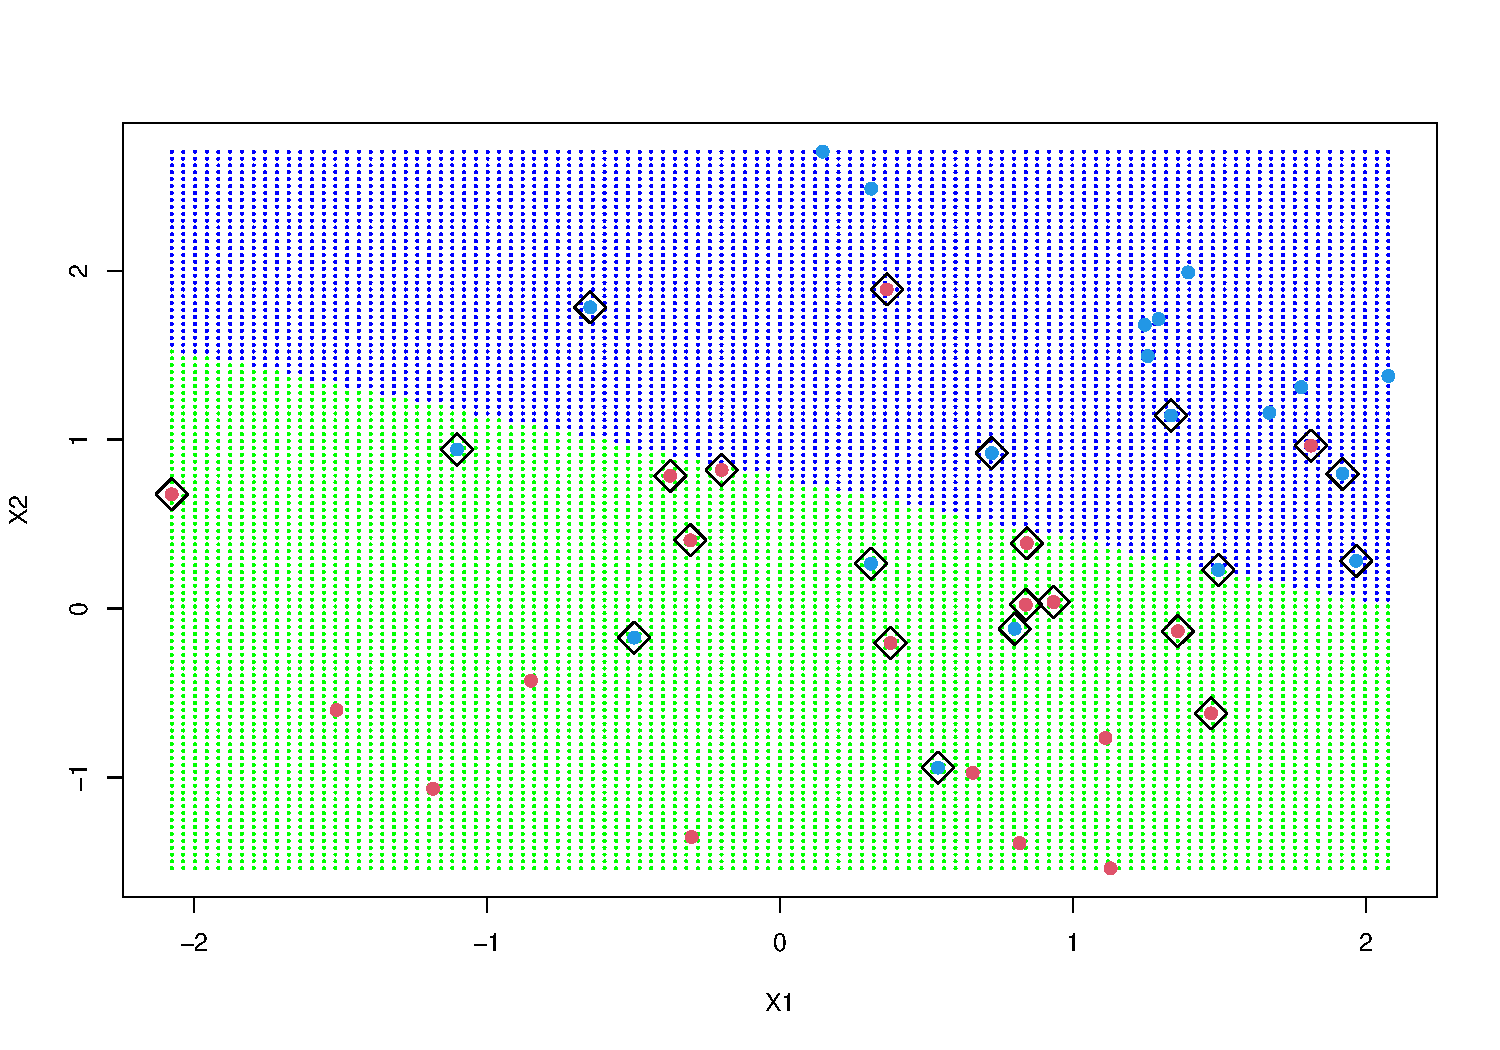
\includegraphics{slides_files/figure-beamer/unnamed-chunk-1-3.pdf}

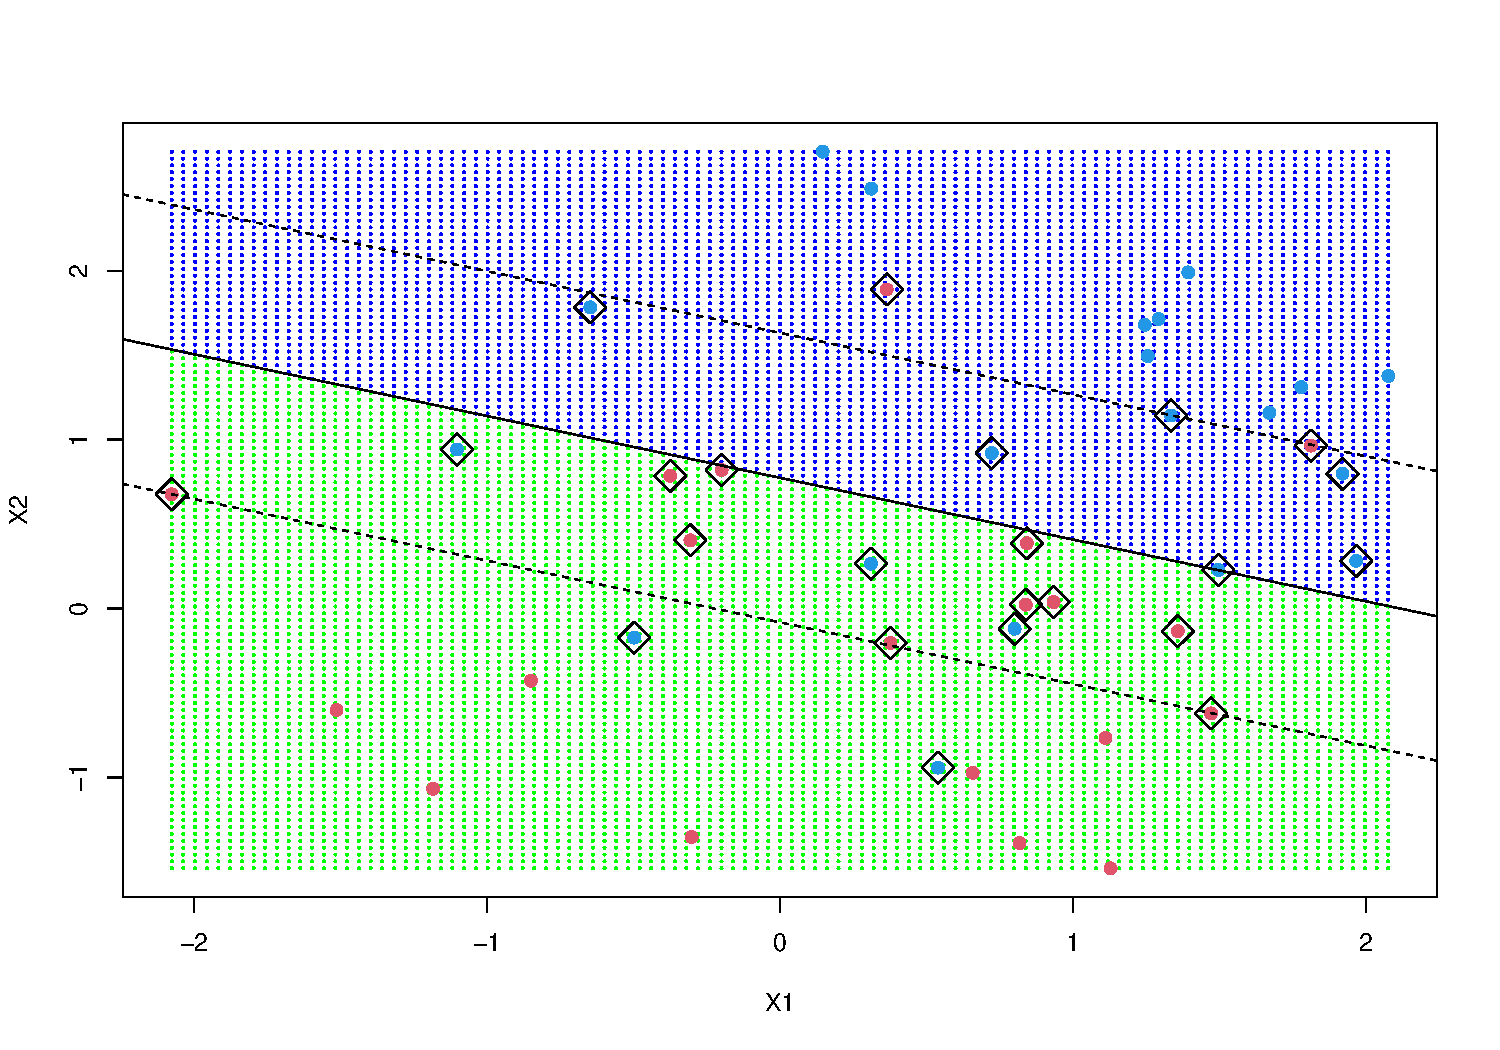
\includegraphics{slides_files/figure-beamer/unnamed-chunk-1-4.pdf}
\end{block}

\begin{block}{Non-Linear Support Vector Machine Classifier}
\protect\hypertarget{non-linear-support-vector-machine-classifier}{}
\end{block}
\end{frame}



\end{document}
